\chapter{Agrupamento}

Com o grande número de serviços prestados em um projeto, surge a necessidade de agrupar essas atividades em grupos de forma a facilitar a identificação com facilidade do grupo de atividades que devem ser executadas para uma determinada finalidade. Um grupo poderá conter outro grupo e/ou serviços ligados à ele.

Um bom exemplo seria a demonstração da imagem \ref{fig:agrupamento}. Nela podemos ver a subdivisão entre grupo, subgrupo e serviços. O grupo, neste caso, seria feito pelo ítem \emph{8 (Instalações Hidrosanitarias/Gas)}, o qual agrupa todos seus serviços ou outros grupos - no caso podem ser demonstrados pelos itens \emph{8.1 (Instalação hidráulica) e 8.2 (Instalações Prediais - Esgoto)}. Dentro dos subgrupos temos os serviços  distribuídos, a exemplo dos itens \emph{8.1.1; 8.2.2; ...; 8.1.12}.

\begin{figure}[htb]
\centering
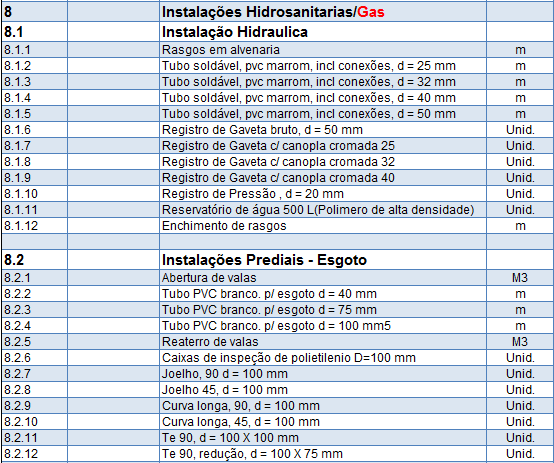
\includegraphics[width=0.7\textwidth]{figuras/agrupamento.png}
\caption{Demonstração de agrupamento de serviços}
\label{fig:agrupamento}
\end{figure}

Sendo assim, um agrupamento pode ter inúmeros outros agrupamentos que, ao final, remetem à um ou mais serviços.